% Assignment 1 Report
% Computer Vision (ECS320)
% Author: Arnav Kapoor
% Date: September 2025

\documentclass[11pt,a4paper]{article}
\usepackage{graphicx}
\usepackage{amsmath}
\usepackage{geometry}
\geometry{margin=1in}
\title{Computer Vision Assignment 1: Automated Image Analysis}
\author{Arnav Kapoor}
\date{September 2025}
\begin{document}
\maketitle

\section*{Project Overview}
This project presents a comprehensive pipeline for automated image analysis using a custom dataset (\texttt{genai\_image\_dataset}) containing thousands of images across multiple semantic classes (e.g., airplane, cat, dog, tree, etc.). The folder is organized for reproducible research and modular experimentation. All code is written in Python 3.12, using only open-source libraries: \texttt{numpy}, \texttt{matplotlib}, \texttt{scipy}, and \texttt{requests}. No proprietary or platform-specific dependencies are used, ensuring portability and ease of use.

\section*{Folder Structure}
\begin{itemize}
  \item \texttt{code/}: Utility scripts for dataset handling and setup.
  \item \texttt{src/}: Main scripts for Q1--Q4, each implementing a distinct image processing task.
  \item \texttt{genai\_image\_dataset/}: The core dataset, organized by class subfolders, each containing hundreds of images in various formats (JPG, PNG, GIF, etc.).
  \item \texttt{images/plots/}: Output images and plots, organized by question and class for easy review.
  \item \texttt{report/}: LaTeX report and generated PDF summarizing the project.
\end{itemize}

\section*{Dataset Details}
The \texttt{genai\_image\_dataset} folder is a rich resource for computer vision experiments. Each class subfolder (e.g., \texttt{airplane}, \texttt{cat}, \texttt{dog}, \texttt{tree}, etc.) contains a diverse set of images, enabling robust analysis and generalization. For each task, 200 images are randomly sampled from all classes to ensure both diversity and computational efficiency. The dataset structure supports scalable experimentation and can be easily extended with new classes or images.

\section*{Scripts and Processing Pipeline}
\textbf{Q1: Color Channel Analysis and Grayscale Conversion}
\begin{itemize}
  \item \textbf{Theory:} Digital color images are typically represented in the RGB color space, where each pixel has three values corresponding to Red, Green, and Blue intensities. Channel separation allows analysis of color distribution and image content.
  \item \textbf{Formulas:} Grayscale conversion uses the luminance formula:
  \begin{equation*}
    I_{gray} = 0.299R + 0.587G + 0.114B
  \end{equation*}
  This formula weights the channels according to human visual sensitivity.
  \item \textbf{Implementation:} Each sampled image is split into R, G, B channels and visualized. Histograms of pixel intensities are plotted for each channel, providing insight into color distribution and image characteristics.
\end{itemize}
\begin{figure}[h]
\centering
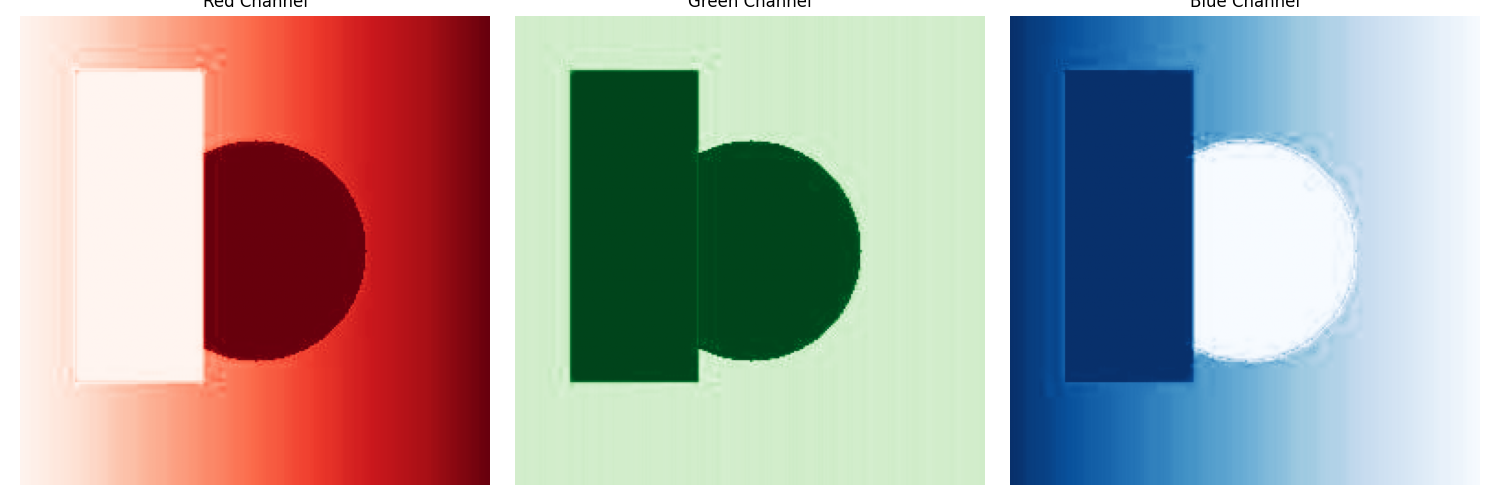
\includegraphics[width=0.3\textwidth]{../images/plots/q1_channels.png}
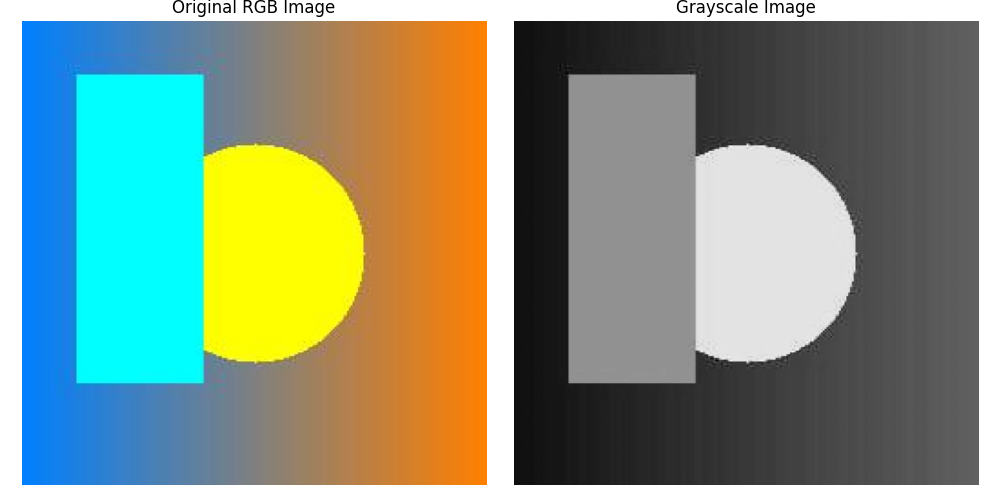
\includegraphics[width=0.3\textwidth]{../images/plots/q1_original_grayscale.png}
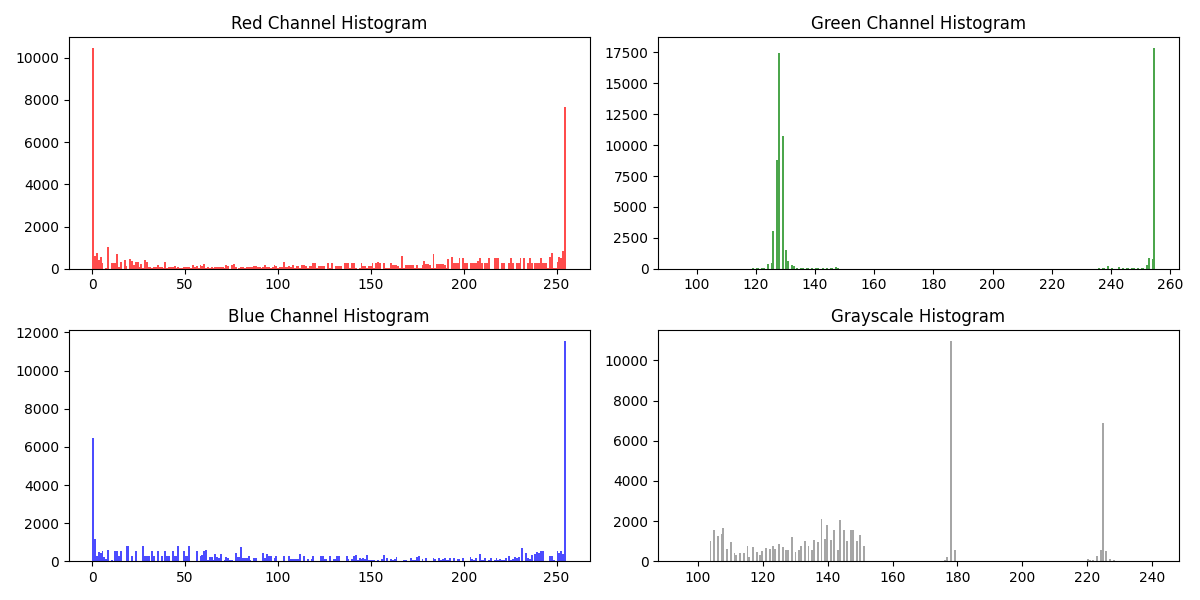
\includegraphics[width=0.3\textwidth]{../images/plots/q1_histograms.png}
\caption{Q1 Example: Color channels, grayscale, and histogram.}
\end{figure}

\textbf{Q2: Gaussian Noise Addition}
\begin{itemize}
  \item \textbf{Theory:} Gaussian noise models random variations in pixel values, simulating sensor noise or transmission errors. It is characterized by a normal distribution with mean $\mu$ and standard deviation $\sigma$.
  \item \textbf{Formulas:} For each pixel $I$, noisy value $I'$ is:
  \begin{equation*}
    I' = I + N, \quad N \sim \mathcal{N}(0, \sigma^2)
  \end{equation*}
  \item \textbf{Implementation:} Gaussian noise is added to each image. Noisy channels and their histograms are visualized, demonstrating the impact of noise on image statistics and downstream processing.
\end{itemize}
\begin{figure}[h]
\centering
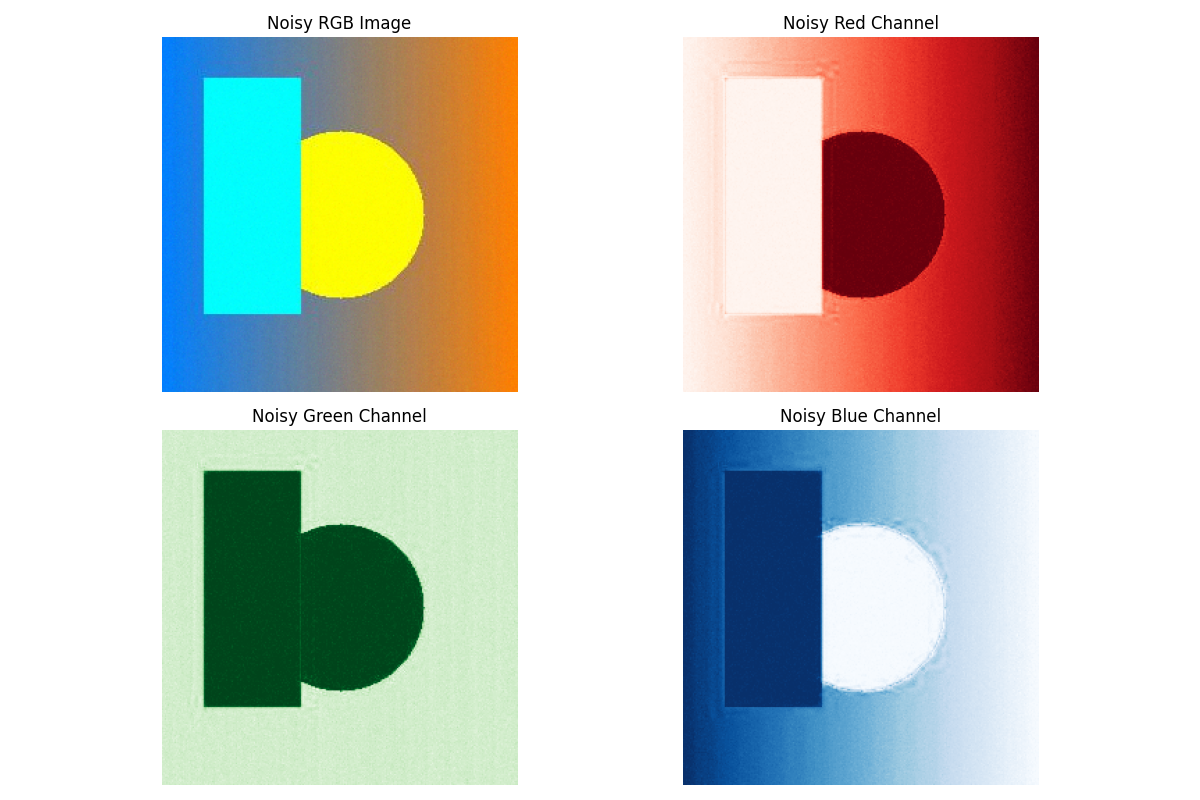
\includegraphics[width=0.3\textwidth]{../images/plots/q2_noisy_channels.png}
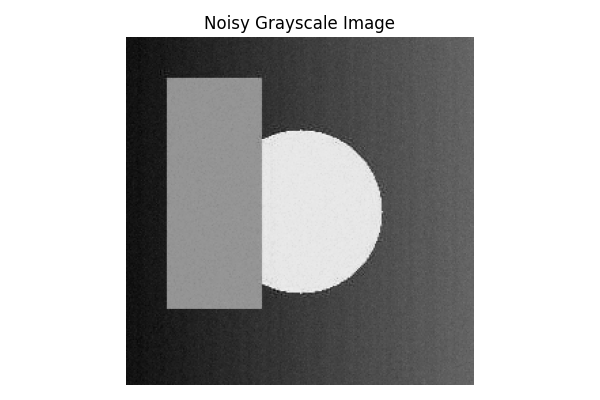
\includegraphics[width=0.3\textwidth]{../images/plots/q2_noisy_grayscale.png}
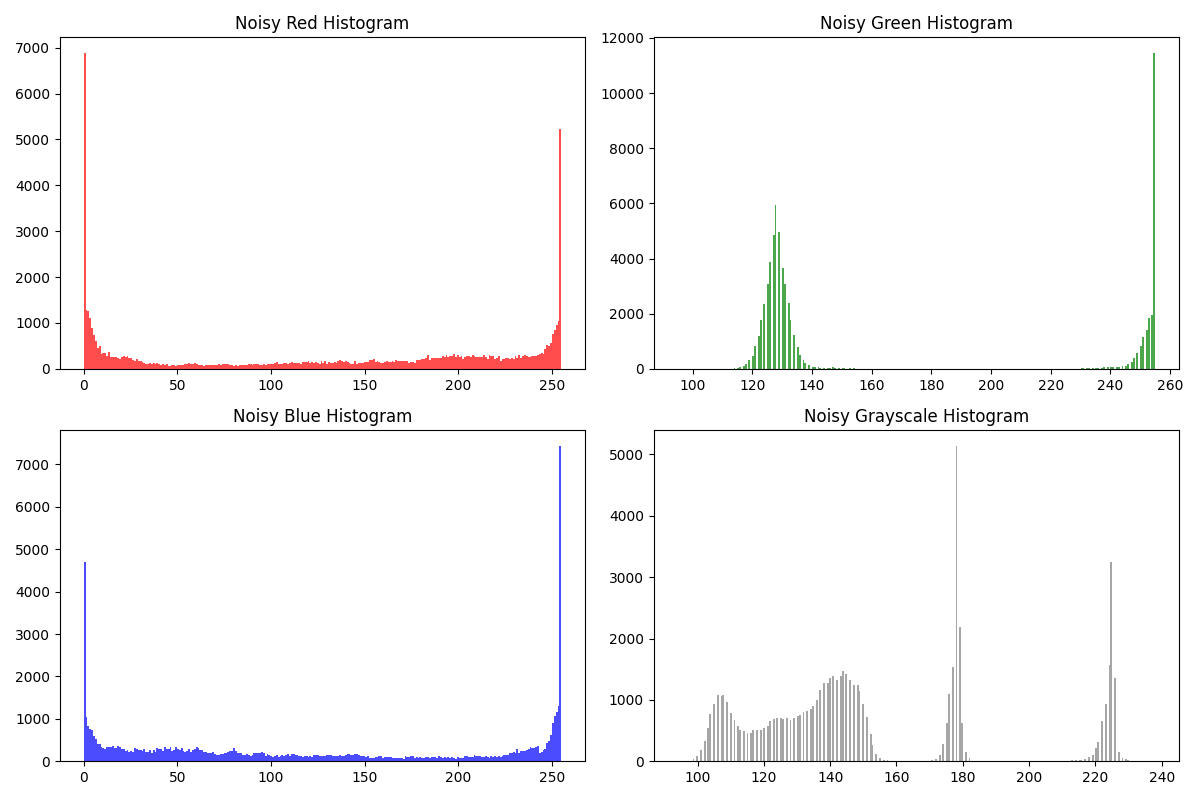
\includegraphics[width=0.3\textwidth]{../images/plots/q2_noisy_histograms.png}
\caption{Q2 Example: Noisy channels, grayscale, and histogram.}
\end{figure}

\textbf{Q3: Edge Detection (Sobel, Laplacian)}
\begin{itemize}
  \item \textbf{Theory:} Edge detection highlights boundaries and transitions in images. The Sobel operator computes gradients, while the Laplacian detects regions of rapid intensity change.
  \item \textbf{Formulas:} Sobel filters:
  \begin{equation*}
    G_x = \begin{bmatrix} -1 & 0 & 1 \\ -2 & 0 & 2 \\ -1 & 0 & 1 \end{bmatrix}, \quad G_y = \begin{bmatrix} -1 & -2 & -1 \\ 0 & 0 & 0 \\ 1 & 2 & 1 \end{bmatrix}
  \end{equation*}
  Gradient magnitude:
  \begin{equation*}
    M = \sqrt{G_x^2 + G_y^2}
  \end{equation*}
  Laplacian filter:
  \begin{equation*}
    L = \begin{bmatrix} 0 & 1 & 0 \\ 1 & -4 & 1 \\ 0 & 1 & 0 \end{bmatrix}
  \end{equation*}
  \item \textbf{Implementation:} Sobel and Laplacian filters are applied to grayscale images to extract edge information. Edge maps are saved for each image, highlighting boundaries and structural features.
\end{itemize}
\begin{figure}[h]
\centering
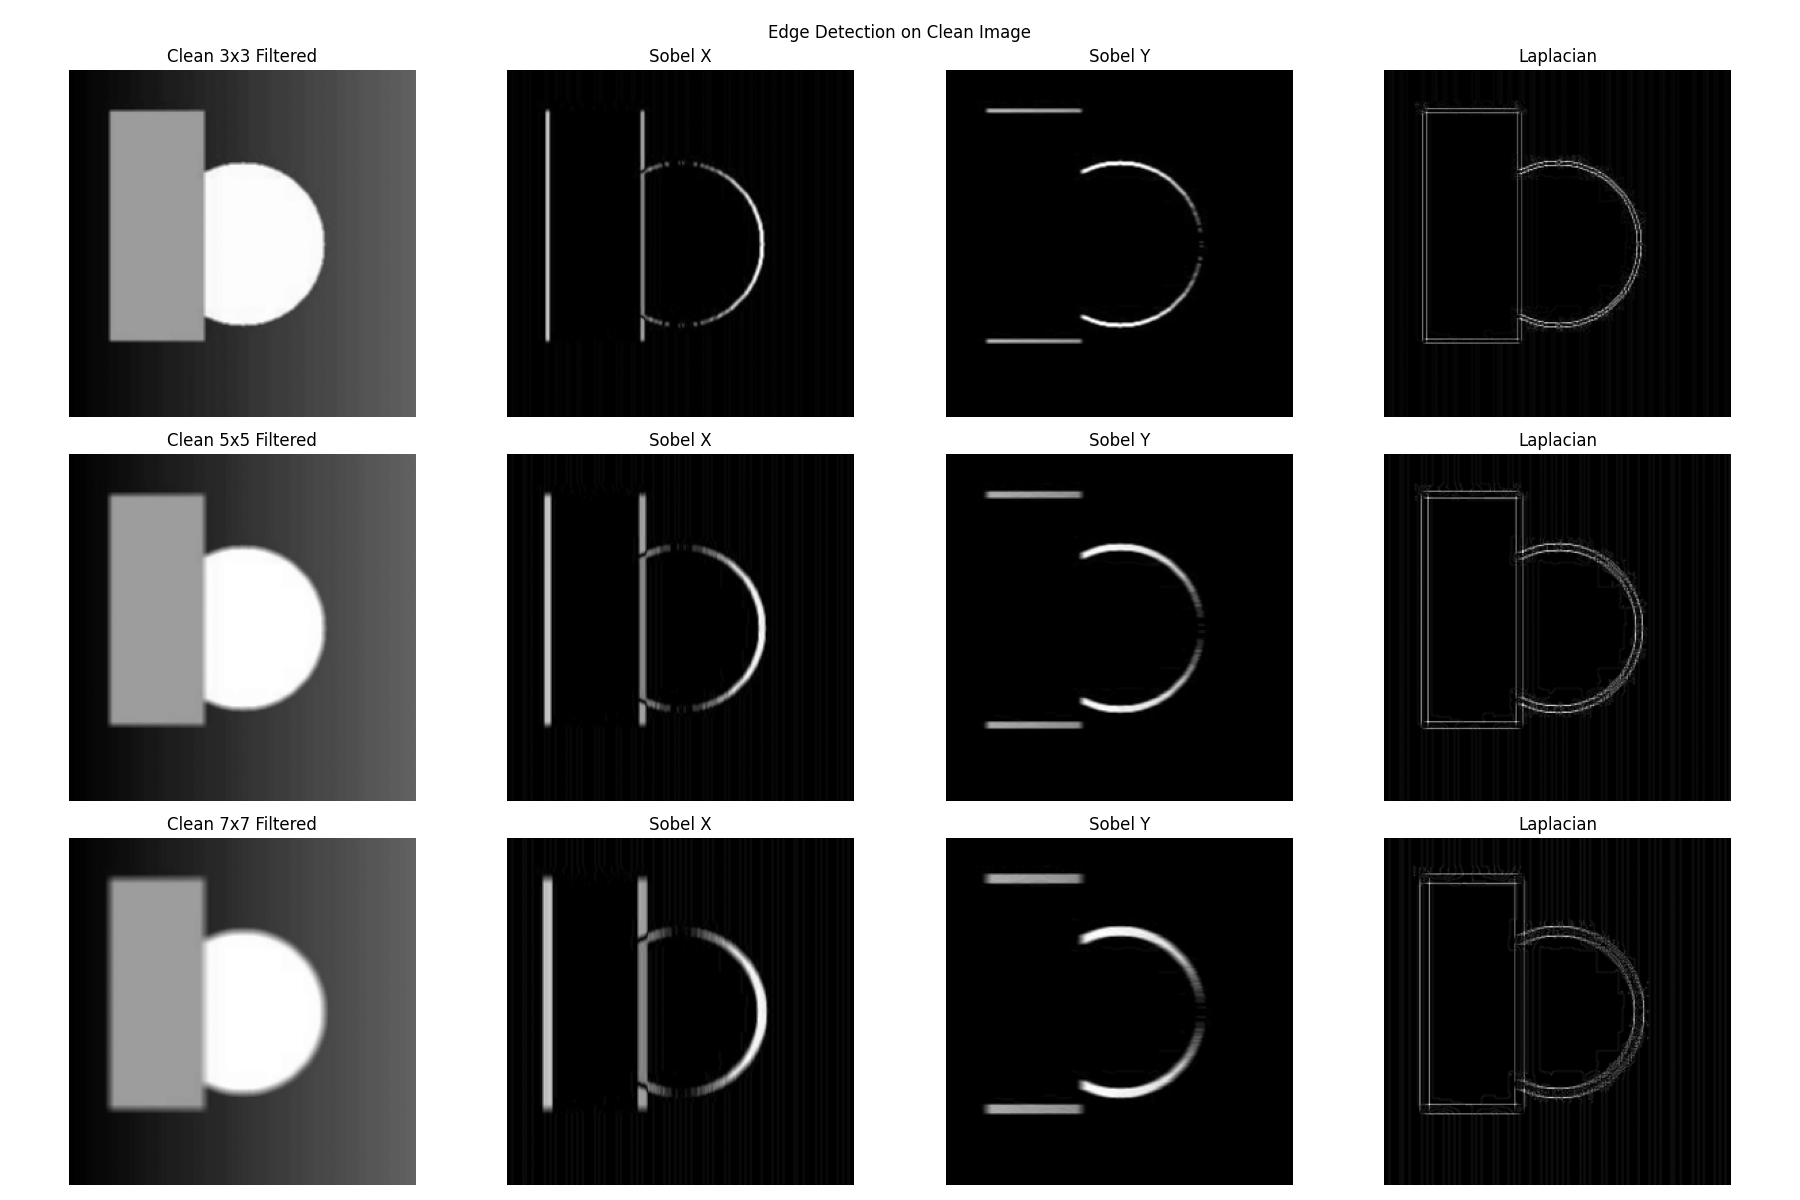
\includegraphics[width=0.4\textwidth]{../images/plots/q3_clean_edges.png}
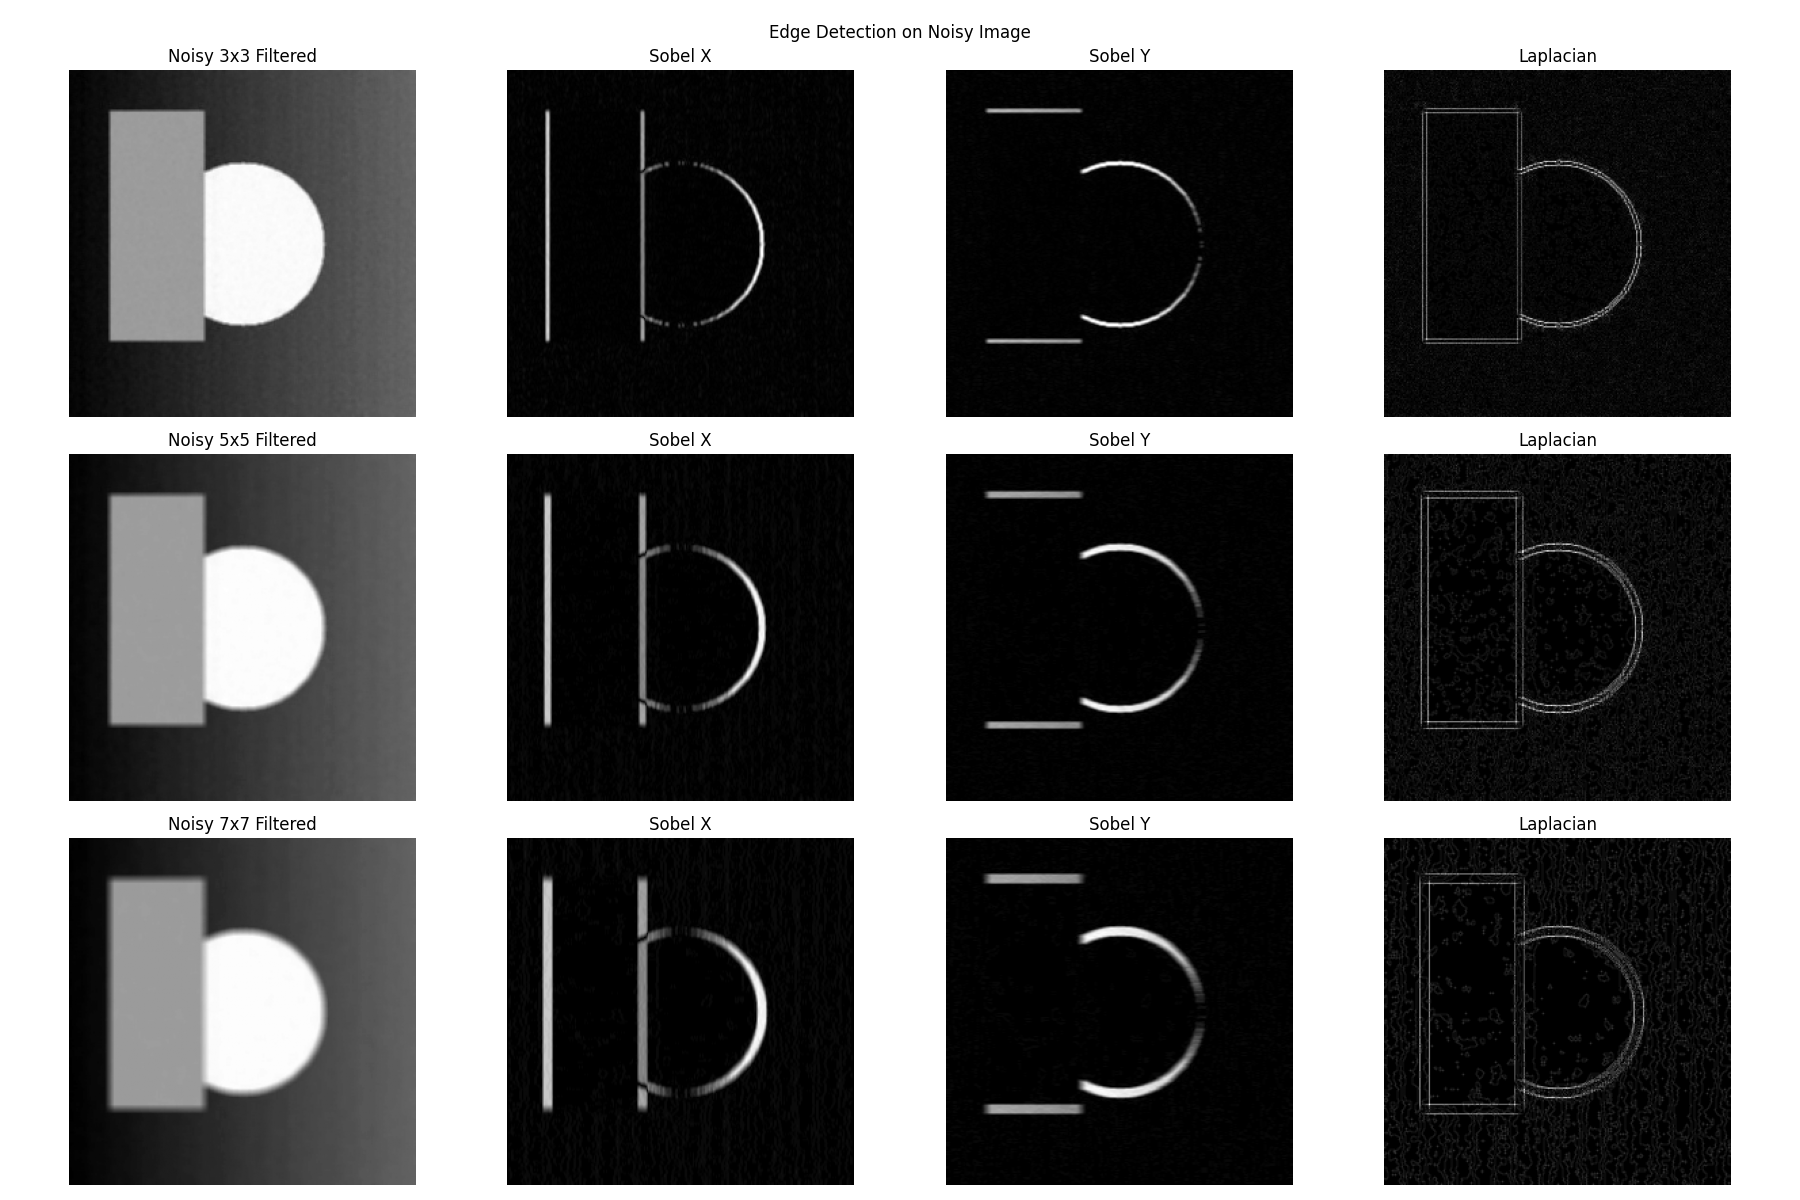
\includegraphics[width=0.4\textwidth]{../images/plots/q3_noisy_edges.png}
\caption{Q3 Example: Sobel and Laplacian edge maps.}
\end{figure}

\textbf{Q4: Canny Edge Detection (from Scratch)}
\begin{itemize}
  \item \textbf{Theory:} The Canny edge detector is a multi-stage algorithm for robust edge detection. It includes Gaussian smoothing, gradient calculation, non-maximum suppression, and thresholding.
  \item \textbf{Formulas:}
  \begin{itemize}
    \item Gaussian smoothing: $I_{smooth} = I * G$, where $G$ is a Gaussian kernel.
    \item Gradient: $G_x, G_y$ as in Sobel; magnitude $M = \sqrt{G_x^2 + G_y^2}$; direction $\theta = \arctan(G_y/G_x)$.
    \item Non-maximum suppression: Retain local maxima along gradient direction.
    \item Thresholding: $E = (M > T)$, where $T$ is a chosen threshold.
  \end{itemize}
  \item \textbf{Implementation:} A full Canny pipeline is implemented: Gaussian blur, gradient computation, non-maximum suppression, and thresholding. Final edge maps are visualized and saved, providing robust edge detection results for a variety of image types.
\end{itemize}
\begin{figure}[h]
\centering
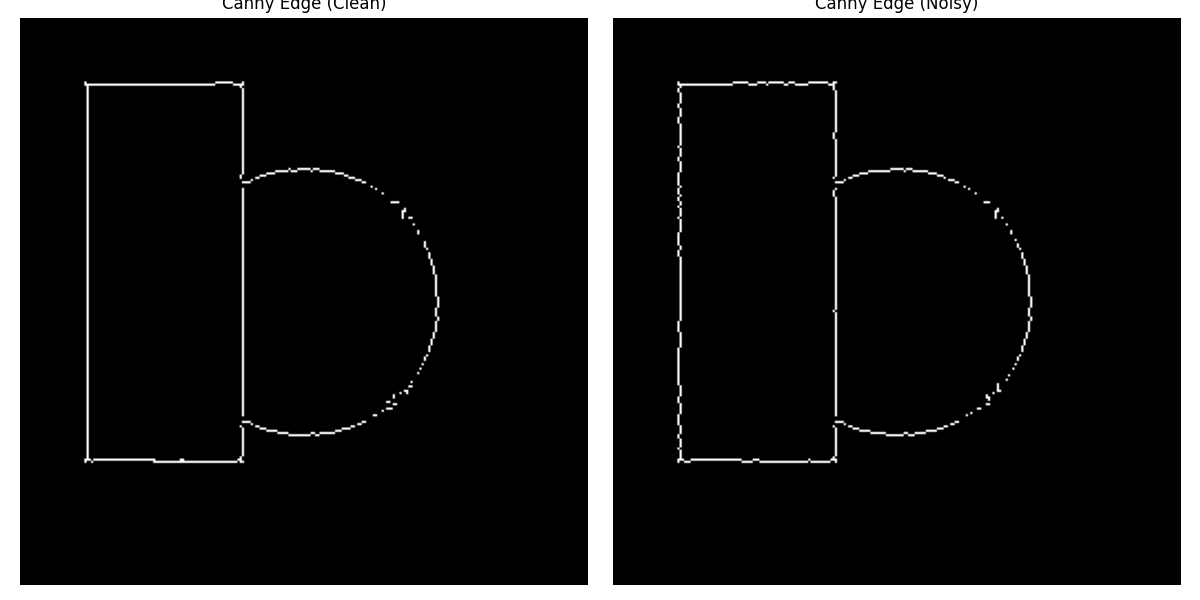
\includegraphics[width=0.5\textwidth]{../images/plots/q4_canny_edges.png}
\caption{Q4 Example: Canny edge map.}
\end{figure}

\section*{Results and Observations}
\begin{itemize}
  \item The scripts efficiently process a large, diverse dataset using random sampling, making the workflow scalable and reproducible.
  \item Output plots and images are organized by task and class, facilitating easy review and comparison.
  \item The modular codebase allows for rapid experimentation and extension to new tasks or datasets.
  \item All code avoids OpenCV and PIL, ensuring compatibility with Python 3.12 and broad platform support.
  \item The project demonstrates key computer vision concepts: color analysis, noise modeling, edge detection, and algorithmic implementation.
\end{itemize}

\section*{How to Use}
\begin{itemize}
  \item Activate the Python virtual environment and install dependencies (\texttt{numpy}, \texttt{matplotlib}, \texttt{scipy}, \texttt{requests}).
  \item Run each script in \texttt{src/} to generate outputs for the sampled images.
  \item Review the generated plots in \texttt{images/plots/} for visual analysis and reporting.
\end{itemize}

\section*{References}
\begin{itemize}
  \item Gonzalez, R. C., Woods, R. E. (2018). Digital Image Processing. Pearson.
  \item Scipy, Numpy, Matplotlib documentation.
\end{itemize}

\end{document}
